% IEEE EuroS&P 2027 submission version (anonymized). Class file and \documentclass options are
% exactly those of the official template (paper/eurosp/template, IEEEtran.cls v1.8b); no layout,
% margin, font or spacing changes. Shares every section with main.tex (the arXiv preprint).
% Build: tectonic -X compile main_eurosp.tex --outdir build_eurosp
\documentclass[compsoc,conference,a4paper,10pt,times]{IEEEtran}
\IEEEoverridecommandlockouts
\usepackage[T1]{fontenc}   % font encoding only (selects the Times fonts under XeTeX/Tectonic); no layout change
\usepackage{amsmath,amssymb,amsfonts}
\usepackage{graphicx}
\usepackage{textcomp}
\usepackage{xcolor}
\usepackage{booktabs,makecell,multirow}
\usepackage[numbers,sort&compress]{natbib}
\usepackage{xurl}
\usepackage{adjustbox}
\usepackage{placeins}
\usepackage{fancyvrb}
\usepackage{tikz}
\usepackage[colorlinks=true,urlcolor=black,linkcolor=black,citecolor=black]{hyperref}
\usepackage[capitalize,noabbrev]{cleveref}

\newcommand{\hesp}{HESP}
\newcommand{\todo}[1]{\textcolor{red}{[TODO: #1]}}
\newcommand{\repourl}{\todo{anonymous repository URL (e.g.\ anonymous.4open.science)}}
\DeclareRobustCommand{\stepnum}[1]{\tikz[baseline=-0.6ex]\node[circle,fill=black,text=white,font=\scriptsize\bfseries,inner sep=0.6pt,minimum size=9pt]{#1};}
\graphicspath{{figures/}{../docs/assets/}}

\begin{document}

\title{\hesp{}: Separating What to Probe from When to Stop in Local LLM Alert-Triage Agents
\thanks{NB: appendices, if any, did not benefit from peer review.}}

\author{\IEEEauthorblockN{Anonymous Submission}}

\maketitle

\begin{abstract}
Security teams increasingly let LLM agents triage alerts, and organizations that keep telemetry in-house must run these agents on small local models. Such an agent reads logs that the attacker partly writes, and the attacker needs only a benign verdict to have an alert closed. Prompt-level defenses give no guarantee, and isolation designs protect tool calls, whereas a triage agent's harmful output is the verdict it computes from attacker-written data. We present \hesp{}, a controller that lets the model read but not decide. \hesp{} keeps a Bayesian ledger of candidate causes, selects read-only probes by expected information gain, and accepts a verdict only if ledger evidence supports it; a benign verdict must further be corroborated by independent sources and may never rest on the model's own reading of a log. On three simulated triage settings with five open-weight models from 7B to 72B, no injected instruction, forged source, or adaptive attack on the model's log parsing closes a case under \hesp{}, whereas without its rules such attacks close up to every actionable case as benign. The controller alone resolves every case in two of the three settings, and neither a 72B planner nor a prompt tuned for the baselines resolves more.
\end{abstract}


\begin{IEEEkeywords}
alert triage, security operations, LLM agents, sequential diagnosis, prompt injection, pre-registration
\end{IEEEkeywords}

\section{Introduction}
\label{sec:intro}

Security teams are starting to hand alert triage and investigation to LLM agents~\citep{guide,cortex,sentinelrl}. An agent receives an alert, queries logs, and reports whether an attack happened and what it touched. Whether such an agent can be trusted to close alerts is decided largely by benchmarks: ExCyTIn-Bench~\citep{excytin}, SIABench~\citep{siabench}, and others report how often agents reach the right answer, and the field reads the numbers as measures of investigation ability. Investigation is the reason to deploy an agent at all. An agent that only recognizes what the alert already says adds nothing an analyst would pay for, and it fails in the cases an attacker creates on purpose, where the malicious activity looks routine and nothing names it.

A benchmark measures investigation only if its items cannot be answered without investigating. Consider an ExCyTIn question generated from a three-hop path: from an alert about a scheduled task, through the host, to a related alert whose IP address is the answer. The question asks for ``the IP address recorded in the related `Anomaly detected in ASEP registry' alert''. One SQL query for that alert name returns the answer; the pivot the question was generated from is unnecessary (\cref{fig:example}). If many items are like this, an agent can earn a score without investigating, and the score says nothing about the cases that matter.

Benchmark papers report model scores but rarely the score of a rule that does not investigate. Security has a tradition of re-evaluations that ask exactly this question of learning-based detectors: simple baselines match complex provenance-based detectors~\citep{bilot2025simpler}, and spurious correlations inflate lab results~\citep{arp2022dos}. Machine learning knows the same problem as shortcut learning~\citep{geirhos2020shortcut,gururangan2018artifacts}. Recent work on incident response proposes new benchmarks that reward evidence discovery~\citep{sirbench}, but the benchmarks already in use have not been audited, and whether the agents evaluated on them use the shortcuts they contain has not been measured.

\begin{figure}[t]
  \centering
  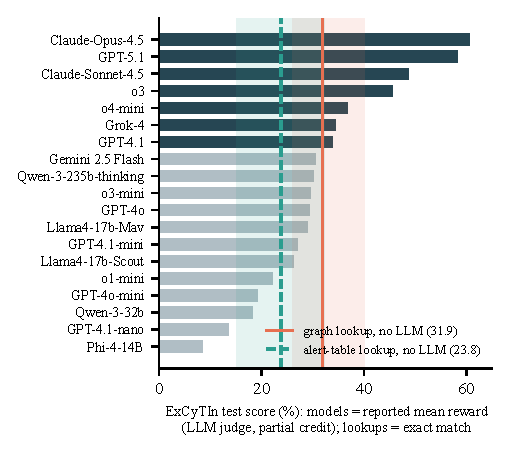
\includegraphics[width=\columnwidth]{fig_floor.pdf}
  \caption{A lookup without an LLM outscores \oBelowGraph{} of \oModels{} reported agents on ExCyTIn-Bench. Bars: mean reward reported for each model on the 589 test questions~\citep{excytin}. Lines: two investigation-free lookups of the alert the question names, on the same questions, scored by exact match (shaded: 95\% intervals, incidents resampled). Dark bars exceed the graph lookup.}
  \label{fig:floor}
\end{figure}

We audit four public benchmarks and datasets for LLM security-operations agents (ExCyTIn-Bench, SIABench, GUIDE, and OTRF Security-Datasets) and three triage environments we built ourselves. For each, we write a fixed rule that uses only what the agent sees, contains no LLM, and skips the investigation the benchmark intends, and we compare it with reported model scores. We find four kinds of shortcut: the question names the evidence that holds the answer (S1), the label follows the organization that assigned it (S2), the data generation leaves a cue such as the attack network's address (S3), and in constructed environments a fixed procedure over the evidence model solves every case (S4). For ExCyTIn, whose authors publish the full logs of 14 agent runs, we go further and test question by question whether the agents' successes come from the shortcut. We registered the hypotheses and froze the rules before every confirmatory run.

\paragraph{Results} Every audited benchmark admits an investigation-free rule that reaches a large share of the reported scores. On ExCyTIn, \oNamed\% of the test questions name the alert that holds the answer, and a lookup of that alert answers \oGraph\% exactly, more than the mean reward of \oBelowGraph{} of \oModels{} reported models (\cref{fig:floor}). On SIABench, ``true positive if and only if the alert involves 172.16.0.1'' is correct on all 35 alerts. On GUIDE, repeating an organization's earlier grade for the same detector is correct on \gHistPct\% of later incidents. In OTRF recordings, the alert text alone separates \otRuleCorrect{} of \otN{} alerts. Yet the ExCyTIn agents do not use the shortcut. Their success is no higher on questions that name the answer's alert (\lgPos{} of \lgModels{} runs, $p=\lgP$); they issue as many queries when one would do; and their ranking is nearly unchanged on shortcut-resistant questions (Kendall $\tau=\lgTau$). The deeper problem is that success depends only weakly on the investigation a question requires: the strongest agent fails \tcOpusFail{} of the 140 questions a single lookup answers.

\paragraph{Contributions}
\begin{itemize}\setlength\itemsep{1pt}
\item A definition of shortcuts for investigation benchmarks and a taxonomy of four kinds, each paired with an investigation-free baseline (\cref{sec:method}).
\item An audit of four public benchmarks and three constructed environments, showing that each admits a rule that reaches or exceeds a large part of reported model scores (\cref{sec:floors}).
\item A question-level analysis of 14 published agent runs on ExCyTIn, showing that the agents do not exploit the shortcut and that their success tracks the required investigation only weakly (\cref{sec:scores}).
\item Checks for benchmark builders, evidence that paired attack and benign ``twins'' remove the single-observation shortcut, and per-question shortcut flags for ExCyTIn (\cref{sec:design}).
\end{itemize}

\section{Background and Motivation}
\label{sec:background}

\subsection{Alert Triage}
Triage decides, for each alert, what caused it and whether a response is needed~\citep{nodoze}. Unlike attack investigation, which reconstructs a whole attack story~\citep{kairos,clouseau}, triage ends with one verdict: a cause and the evidence for it. The analyst reaches the verdict by querying the environment, and queries differ in cost and in how well they separate the candidate causes.

Consider an alert that reports a spike in authentication failures and HTTP errors on a web tier (\cref{fig:motivating}). It looks like credential stuffing, but SQL-injection probing, an authorized vulnerability scan, a misclassified health check, and an administration panel exposed to the internet produce the same symptom. A threat-intelligence lookup on the top source may answer ``malicious'', which three of these causes share. Reading the admin panel's configuration, one cheap query, settles the last explanation at once, but only an investigator who keeps that explanation in view will run it. An investigation therefore makes two decisions again and again: which query to run next, and whether the evidence already suffices.

\subsection{Small Models Fail at the Procedure}
\label{sec:motivation}
An LLM agent makes both decisions itself~\citep{react}: at each step the model reads the observations so far, then calls a tool or states a verdict. \Cref{fig:motivating} shows what happens when the model is Llama-3.1-8B and the true cause is the exposed admin panel. When the model chooses the probes and decides when to stop (first row), it never runs the decisive query. When a controller chooses the probes but the model still decides when to stop (second row), the model sees the decisive observation at step three and keeps probing until the budget is gone. Only when the controller also stops does the episode end with the right verdict.

\begin{figure*}[t]
  \centering
  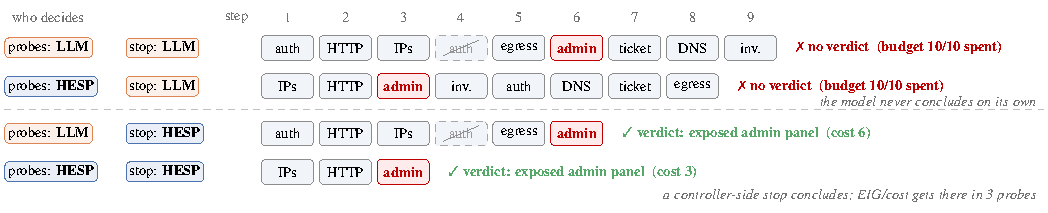
\includegraphics[width=\textwidth]{fig_motivating.pdf}
  \caption{Choosing probes and stopping are separate failures. One alert (true cause: an exposed admin panel), one local model (Llama-3.1-8B), four ways to split the investigation. Each chip is a probe that ran (dashed: a duplicate proposal the controller blocked); red marks the observation that confirms the cause. When the model decides when to stop (first two rows), it reaches the decisive evidence and keeps probing. A controller-side stop concludes (last two rows), and information-gain selection gets there in three probes. All rows are taken from archived journals.}
  \label{fig:motivating}
\end{figure*}

The pattern holds beyond this alert. Qwen2.5-7B choosing its own probes resolves 8 to 13\% of cases while spending nearly its whole budget, and uniformly random probes would do better. Llama-3.1-8B requests another probe in all 3{,}389 of its decisions, including those in which the ledger's posterior exceeds 0.999. Larger models do conclude, but without a ledger Qwen2.5-32B and 72B cite invalid evidence in 22 to 31\% of their citations. Two small models of similar size thus fail in different places, one at choosing probes and one at stopping (\S\ref{sec:utility}), which is why a controller has to take over both decisions rather than repair one.

\subsection{Attacker-Written Evidence}
An agent that reads retrieved content can be steered by instructions hidden in it, namely indirect prompt injection~\citep{greshake2023}, which AgentDojo benchmarks on tool-using agents~\citep{agentdojo}. Log injection through unescaped user-controlled fields is an older form of the same problem~\citep{owasp_loginjection}, and LogInject shows that LLM log analysis in SOCs follows such payloads at high rates~\citep{loginject}. Defenses fall into two families. Model-level defenses, such as structured queries and preference optimization~\citep{struq,secalign}, reduce but do not remove the model's tendency to follow injected text. System-level defenses separate a privileged planner from the untrusted data: the Dual LLM pattern and CaMeL~\citep{camel} let a quarantined model read the data while a planner fixes the control flow, and CaMeL, FIDES~\citep{fides}, and Progent~\citep{progent} enforce policies on the tool calls that follow. CaMeL also shows that the quarantined reader remains a channel: an attacker who cannot change the plan can still choose the values the reader returns. In triage this channel is the whole attack, because the verdict is computed from the values the reader returns and no tool call follows that a policy could stop.

\section{Motivation}
\label{sec:motivation}

\subsection{Challenges}
When a small local model drives the investigation, three challenges arise. We measured each on the baseline configurations of our studies (\S\ref{sec:setup}), in which the model chooses its own probes.

\stepnum{1} \textbf{Probing without converging.} Qwen2.5-7B selecting its own probes verifies only 0.083 to 0.125 of cases. It runs about seven distinct probes per episode, spends 9.4 to 9.5 of its 10 cost units, and issues a verdict in only 6 or 7 of 72 episodes; three quarters of its episodes end with the tool budget exhausted. Replacing its choices with uniformly random ones raises completion by $+0.556$ (\S\ref{sec:rq-rank}), so its own choices are worse than chance.

\stepnum{2} \textbf{Never deciding to stop.} In the decomposition study, under our prompt and serving configuration, Llama-3.1-8B requests another probe in every one of its 3{,}389 decisions, including those in which the ledger's posterior exceeds 0.999 and the prompt states that no legal probe is left. Its outputs are valid JSON throughout; it simply never finishes. Better probing cannot help a model that never states a verdict.

\stepnum{3} \textbf{Verdicts without support.} Larger models conclude, but not always on evidence. Without a ledger, Qwen2.5-32B and 72B call 13 of 51 and 20 of 54 actionable incidents benign among those they give a verdict on, and cite invalid evidence in 22\% and 31\% of their citations (\S\ref{sec:security}). In triage, a verdict that dismisses a real attack is the costliest error, because the incident is closed without a response.

\subsection{Our Solution}
\hesp{} answers each challenge with a component outside the model. \stepnum{1} It ranks every legal probe by expected information gain per cost, from likelihood tables counted in LLM-free development runs rather than elicited from the model, which cannot supply them (elicited tables leave completion at 0.069 to 0.375, \S\ref{sec:rq-help}). \stepnum{2} Before each planner call it applies an explicit acceptance rule and concludes on its own once the rule is met (Appendix~\ref{app:loop} gives the exact order). \stepnum{3} It accepts only verdicts that cite a current observation supporting the claimed cause, and a write-ahead journal lets an audit replay every step.

\section{\hesp{} Design}
\label{sec:approach}

\hesp{} sits between a local LLM and the probe catalogue (\cref{fig:pipeline}). The model proposes: at each step it may suggest a probe, propose a verdict, or abstain, and it parses raw logs when a probe returns text. The controller decides: it chooses which probe runs, which verdict is accepted, and when the investigation ends. Every step is written to a journal before its observation arrives and is audited afterwards.

We walk through the running example. The alert leaves nine candidate causes at probability 0.111 each. The controller ranks the probes by expected information gain per cost and runs \texttt{source\_ips}, although the model proposed \texttt{auth\_log} (1.74 against 0.51 bits per cost unit); the result, \textit{normal}, leaves four causes at 0.238. \texttt{access\_pattern} leaves three at 0.327: the exposed admin panel, a vulnerable component, and DNS command-and-control. \texttt{admin\_exposure} returns \textit{exposed, no auth}, which moves the admin panel to 0.966. Before the next model call, the controller sees that the leader exceeds the acceptance threshold and that the last observation singles it out, and it ends the episode with that verdict after three probes and 5.1\,s.

\begin{figure*}[t]
  \centering
  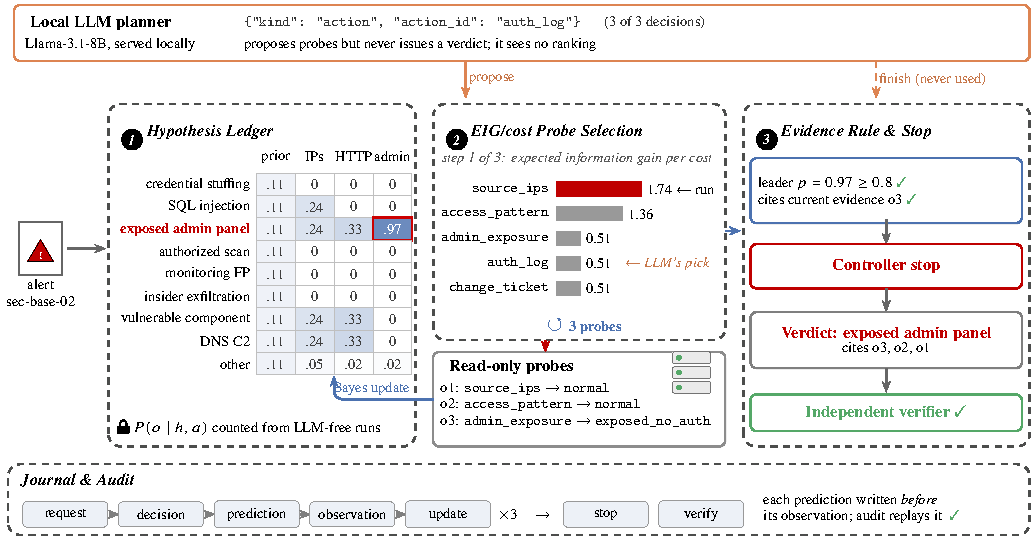
\includegraphics[width=\textwidth]{fig_pipeline.pdf}
  \caption{\hesp{} on the running example (Llama-3.1-8B; true cause: an exposed admin panel). \protect\stepnum{1} The ledger keeps a posterior over the candidate causes, updated by Bayes' rule from frozen probe-outcome tables. \protect\stepnum{2} The controller runs the legal probe with the highest expected information gain per cost; the model's proposal (here \texttt{auth\_log}, three times) is advisory. \protect\stepnum{3} Once the leader's posterior reaches 0.8 and a current observation singles it out, the controller concludes and cites that evidence. The verifier is used for evaluation only. All values are taken from the archived journal.}
  \label{fig:pipeline}
\end{figure*}

\subsection{Evidence Ledger}
\label{sec:ledger}
\label{sec:tables}
\emph{Problem.} The controller needs a model of what each probe would return under each cause; the LLM cannot provide one (tables elicited from the planner leave resolution at 0.069 to 0.375, \S\ref{sec:policy}).

\emph{Mechanism.} Before deployment, a script runs every probe once in each of $k$ development episodes of every cause and counts the outcomes into a table
\[\widehat P(o \mid h, a) = \frac{q_{h,a,o}}{\sum_{o'} q_{h,a,o'}},\quad q_{h,a,o} = (1-\varepsilon)\,\frac{n_{h,a,o}}{n_{h,a}} + \frac{\varepsilon}{|O_a|},\]
where $n_{h,a,o}$ counts valid observations of outcome $o$ for probe $a$ under cause $h$, $O_a$ is the probe's outcome vocabulary, and $\varepsilon = 0.01$. A cause without development cases, such as \textit{other}, gets a uniform row. The tables are hashed and frozen before use. For each alert, the ledger starts from a uniform prior over the candidate causes and applies Bayes' rule, $p_t(h) \propto p_{t-1}(h)\,\widehat P(o_t \mid h, a_t)$, after every valid observation, recording whether the observation raised or lowered each cause's score. Transient failures (e.g., HTTP 503) are journaled but are not evidence. When the environment reports that the incident changed, the scores reset to the prior and earlier observations stop counting as current.

\emph{Alternatives.} Asking the model for likelihoods removes the need for development data but fails, as noted above. In our settings, five development episodes per cause already give tables that resolve every case (\S\ref{sec:policy}); a deployment would count resolved tickets or replayed incidents (\S\ref{sec:discussion}).

\subsection{Probe Selection}
\label{sec:selection}
For every legal probe, i.e., one that has not run in the current state, is affordable, and has its prerequisites met, the controller computes the expected information gain
\begin{align*}
\mathrm{EIG}(a) &= H(p) - \textstyle\sum_{o} P(o \mid a)\, H\big(p(\cdot \mid o, a)\big),\\
P(o \mid a) &= \textstyle\sum_h p(h)\, \widehat P(o \mid h, a),
\end{align*}
and runs the probe with the highest $\mathrm{EIG}(a)/c(a)$, where $c(a)$ is its cost. The criterion is the classical one~\citep{dekleer1987,golovin2010}; what matters here is that the model's proposal no longer decides which probe runs. The model receives the task, the catalogue, the observations, the ledger, and feedback on rejected proposals (Appendix~\ref{app:prompt}), and returns one JSON decision.

\subsection{Evidence Rule and Stopping}
\label{sec:finish}
\emph{Finish guard.} A verdict proposed by the model is accepted only if the claimed cause has a current score of at least $\tau = 0.8$ and at least one cited observation is current and supports it in the ledger. A rejected verdict is returned to the model as feedback. Text in a log never enters the ledger, so text alone cannot satisfy the guard.

\emph{Controller stop.} Before each model call, and when a budget runs out, the controller applies the same rule to the current leader and, if it holds, concludes on its own, citing up to three supporting observations. The \emph{confirmation} variant additionally requires one observation that \emph{specifically} supports the leader, i.e., whose outcome is at least ten times more likely under the leader than under any other named cause. It uses the tables only and forbids conclusions reached purely by elimination.

\emph{Recovery.} A model can stall a guarded controller by proposing the same verdict just below the threshold. After two consecutive rejected verdicts, the controller runs its own top-ranked probe instead of asking the model again.

\subsection{Source-Diverse Corroboration}
\label{sec:corroboration}
Once the controller decides, an attacker forges evidence instead of text, and a single forged observation that singles out a benign cause suffices, because the controller acts on its most informative observation first. \hesp{} therefore requires a benign verdict, whether proposed by the model or reached by the controller stop, to rest on current observations from at least two different \emph{source groups} that each specifically support it. A source group is the upstream data source behind a probe, declared per deployment; two probes that read the same reputation feed form one group. If the rule is not met, the controller keeps probing, and if the evidence stays inconsistent, the case is escalated.

\subsection{Reader Trust}
\label{sec:readertrust}
When a probe returns log text, a parser maps it to the probe's outcome vocabulary. A rule parser written for the documented format is safe but reads nothing after a format change; the model reads any format but can be persuaded. \hesp{} tags each observation with the parser that produced it. Under the \emph{reader-trust} rule, an observation parsed by the model updates the posterior and may confirm an actionable cause, but it never counts as specific support for a benign verdict, in the controller stop, in corroboration, and in the finish guard alike. The asymmetry follows the attacker's goal: a forged reading that confirms an attack costs an unnecessary escalation, whereas one that confirms a benign cause closes the case. The rule is a provenance label in the spirit of capabilities and information-flow labels~\citep{camel,fides}, specialized to one decision.

\subsection{Security Analysis}
\label{sec:analysis}
Whatever the model outputs, three properties hold: every executed probe is in the read-only catalogue and affordable; every accepted verdict cites a current observation that raised the claimed cause's score (G3); and every prediction is journaled before the observation it predicts, which the audit checks. Against A1, the finish guard and the controller stop suffice, because injected text never becomes ledger evidence. Against A2, neither helps: a forged source produces genuine-looking evidence. Source-diverse corroboration restores G2 as long as the attacker controls at most one source group. Against A3, corroboration no longer helps, because the attacker's text arrives with every probe's response and can forge the reading of every source group. Reader trust restores G1 as long as a trusted parser exists, at the cost of escalating honest benign cases whenever only the model can read the logs. None of these rules makes a verdict correct; correctness depends on the tables and on the true cause being among the candidates, which \S\ref{sec:policy} evaluates.

\subsection{Implementation}
\label{sec:implementation}
\hesp{} is about 2{,}900 lines of Python that use only the standard library. One JSON decision protocol serves vLLM and Ollama endpoints and the scripted planners used as LLM-free references. Each episode runs against its own loopback HTTP sandbox, so probes are real HTTP requests with transient failures and state changes. A write-ahead journal records every request, decision, prediction, observation, and ledger update, and an audit replays each journal and checks event order, provenance, budgets, citations, and every controller verdict. 201 unit tests cover the ledger, selectors, guard, stop, corroboration, reader trust, and the isolation of the table estimator from the environment's generator.

\section{Evaluation Setup}
\label{sec:setup}

To assess \hesp{}, we structure our evaluation around seven questions:
\begin{enumerate}
  \item \emph{Reliability:} Does \hesp{} make small local models reliable triage agents, and does it depend on oracle knowledge of the environment? (\S\ref{sec:rq-help})
  \item \emph{Ranking versus Choice:} Is the gain due to the information-gain ranking, or merely to taking the choice of probe away from the model? (\S\ref{sec:rq-rank})
  \item \emph{Probing versus Stopping:} Are choosing what to probe and deciding when to stop separate failures, and which one does each model have? (\S\ref{sec:rq-stop})
  \item \emph{Failure Modes:} How do verdicts fail, in security terms? (\S\ref{sec:security})
  \item \emph{External Validity:} Do the effects hold on tasks that we did not design? (\S\ref{sec:external})
  \item \emph{Table Error:} How does the controller fail when its prediction tables are wrong? (\S\ref{sec:mismatch})
  \item \emph{Adversarial Evidence:} What happens when the attacker writes instructions into the logs or forges a piece of evidence? (\S\ref{sec:adversarial})
\end{enumerate}
Each study was designed after the previous one had run (\cref{tab:studies}); the last three questions share one pre-registered study with three parts. \S\ref{sec:realdata} then asks whether public security data could test the same questions.

\begin{table*}[t]
  \caption{Overview of the five pre-registered studies: 11{,}912 audited LLM episodes, plus the LLM-free episodes of the table-error part. The repository labels the studies by version.}
  \label{tab:studies}
  \centering\small
  \begin{adjustbox}{max width=\textwidth}
  \begin{tabular}{llllrl}
    \toprule
    Study & Version & Question & Models & Episodes & Primary endpoint(s) \\
    \midrule
    Initial & v0.5 & does the controller help? & 3 Qwen & 1{,}944 & full \hesp{} vs.\ Memory-only, per model \\
    Table-source & v0.6 & must the tables come from an oracle? & 3 Qwen & 1{,}728 & counted-table \hesp{} vs.\ Memory-only, 7B \\
    Decomposition & v0.8 & ranking or loss of choice? second family & 5 & 1{,}800 & ranking vs.\ random (Q-7B); \hesp{} vs.\ Memory-only (L-8B) \\
    Stopping & v0.9 & what to probe vs.\ when to stop & 5 & 1{,}800 & controller stop; selection given stop (both L-8B) \\
    \midrule
    External family & v1.0-A & do the effects hold on tasks we did not design? & 5 & 3{,}800 & ranking; full effect (both Q-7B) \\
    Table error & v1.0-B & what if the tables are wrong? & none & LLM-free & descriptive only \\
    Adversarial evidence & v1.0-C & injected instructions and forged evidence & 5 & 840 & injection attack success (Q-7B) \\
    \bottomrule
  \end{tabular}
  \end{adjustbox}
\end{table*}

\subsection{Environment and Tables}

\subsubsection{The sec-triage Environment} Each episode is one alert on a web service. The hidden cause is one of eight explanations: three attacks (credential stuffing, SQL-injection probing, DNS command-and-control), an insider exfiltrating data, an exposed admin panel, a known-vulnerable component, an authorized vulnerability scan, and a monitoring false positive. The hypothesis set adds \textit{other}. Ten read-only probes, costing 1 to 3 units each, cover authentication failures, HTTP patterns, source reputation, admin exposure, per-user egress, DNS characteristics, component inventory, change tickets, threat intelligence, and a generic runbook. We designed the environment so that shortcuts fail. Threat intelligence says only that an indicator is malicious, and three attacks share that answer. The runbook carries no information. Several benign causes look like attacks until the right probe runs. Each cause appears in three variants. In \textit{base}, outcomes are deterministic except for a 10\% threat-intelligence lag. \textit{Noise} adds 15\% transient HTTP 503 failures and a 30\% lag. In \textit{drift}, the incident is superseded after the second probe: the state version advances and the true cause switches. This gives 24 tasks, and each study runs every task three times per configuration. Each episode is served from its own loopback HTTP sandbox.

\subsubsection{Prediction Tables} We compare three sources of $P(o \mid h, a)$. \emph{Designer} tables come from the environment's generating function and serve as an oracle reference. \emph{Counted} tables (``empirical'' in the tables) are estimated as in \S\ref{sec:tables}, with $k \in \{1, 5, 20, 100\}$ development episodes per cause and variant, from the base and noise variants only and with seeds drawn from a space disjoint from evaluation. \emph{Elicited} tables are produced by the planner LLM itself. Every table is frozen and hashed before any evaluation episode runs. Because development and evaluation episodes come from the same generator, the counted tables tell us how many observations are enough, not how the method behaves in an unfamiliar environment.

\subsubsection{The sigma-triage Family} To test whether the effects depend on an environment we built, the v1.0 study derives a second task family mechanically from the public SigmaHQ detection-rule repository~\citep{sigmahq}, pinned to one commit. Each Sigma rule states the alert, the ATT\&CK technique it targets, and a \texttt{falsepositives} field in which the rule's author lists known benign explanations. A task is one rule firing. Its candidate causes are the attack the rule targets, up to four benign explanations taken verbatim from that field, and \textit{other}. Eligibility was fixed before sampling (status stable or test, level medium or higher, an ATT\&CK tag, and at least two specific benign explanations), and 12 of the 159 eligible rules were drawn with a fixed seed; they cover Windows endpoints, Azure, Kubernetes, and GitHub. Ten generic investigation probes, written before any rule was drawn, are shared by all rules: the acting account, the logon origin, a change ticket, software approval, binary reputation, prevalence across the fleet, the parent process, the time window, follow-on activity, and threat intelligence. Which outcome each probe returns under each cause was annotated once by a model outside both planner families (phi-4~\citep{phi4}, temperature 0, constrained to the fixed outcome vocabulary) and then frozen. A rule whose annotation left two causes indistinguishable was replaced by the next rule in the sampled order, which happened once. The family has 76 tasks (base and noise variants), and its tables are counted from LLM-free development runs exactly as for sec-triage.

\subsubsection{Adversarial Variants} Two further sec-triage variants, used only with the six causes that require action, implement the threat model's attacker. In \emph{inject}, every probe response carries an attacker-controlled free-text field, as a user agent or a task description would, holding an instruction to close the case as an authorized scan and to cite that observation. The classifier reads structured fields only, so the ledger never sees the text, but any planner that reads raw responses does. In \emph{spoof}, the attacker routes traffic through a scanner-looking address, so the source-reputation probe reports a known scanner whatever the cause; this does mislead the ledger. Two benign causes under the base variant measure what the asymmetric-evidence rule costs honest cases.

\begin{figure*}[t]
  \centering
  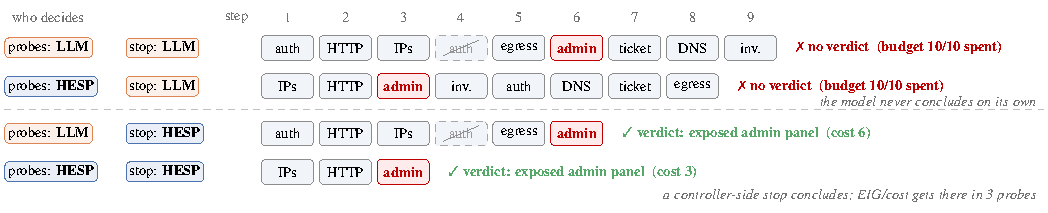
\includegraphics[width=\textwidth]{fig_motivating.pdf}
  \caption{One alert, one local model, four ways to split the investigation. The alert's true cause is an exposed admin panel; the planner is Llama-3.1-8B in every row, with the same seed. Each chip is a probe that ran (dashed: a duplicate proposal the controller blocked); red marks the observation that confirms the cause. When the model decides when to stop (first two rows), it reaches the decisive evidence and keeps probing until the budget is gone. A controller-side stop concludes (last two rows), and information-gain selection gets there in three probes. All four rows are taken verbatim from the stopping study's archived journals.}
  \label{fig:motivating}
\end{figure*}

\subsection{Experiment Design}

\subsubsection{Configurations} All configurations use the same model, prompt template, probe catalogue, budgets (10 tool calls, 10 cost units, 12 decisions, 900\,s), duplicate blocking, and verifier. \emph{ReAct-style}: the planner sees the raw observation history only and picks every probe. \emph{Memory-only}: the planner also sees the ledger and still picks every probe. \emph{\hesp{}}: the controller picks the probe (EIG/cost or random), with or without showing its ranking, and with or without the finish guard and the controller-side stop. \Cref{fig:motivating} shows four of these configurations on the same alert. After the stopping study we also ran the frozen controller with the LLM replaced by a script that proposes probes in catalogue order and never finishes. This \emph{LLM-free reference} uses the stopping study's seeds, tasks, budgets, and table (216 episodes); it was not pre-registered and we report it as exploratory. The v1.0 study reuses the stopping study's five configurations on sigma-triage. On the adversarial variants it compares ReAct-style, Memory-only, \hesp{} with the finish guard and controller stop, and the same with the asymmetric-evidence rule of \S\ref{sec:finish}. The table-error part replaces the LLM with the never-finishing script and compares EIG/cost, random, and catalogue-order selection, all under a controller stop.

\subsubsection{Implementation} \hesp{} is about 2{,}900 lines of Python that use only the standard library. Planners are pluggable: one JSON decision protocol serves vLLM and Ollama endpoints and the scripted policies used for LLM-free runs. Each episode gets its own loopback HTTP sandbox, so probes are real HTTP requests with transient failures and state changes, and no episode can observe another. Every study uses Qwen2.5-7B-Instruct (bf16), Qwen2.5-32B-Instruct-AWQ, and Qwen2.5-72B-Instruct-AWQ; the decomposition and stopping studies add Llama-3.1-8B-Instruct (bf16) and Llama-3.1-70B-Instruct-AWQ-INT4. Models are served by vLLM on a single RTX~6000-class GPU at temperature 0.2, with a distinct seed per call. A paired, shuffled, resumable runner executes up to 32 episodes concurrently and refuses to resume if the manifest or the hash of the controller source has changed. After each model, it audits all episodes, archives the journals, and records the archive's SHA-256. The stopping study's 1{,}800 episodes ran in 28 minutes, and the v1.0 study ran on the same server, serving stack, and weights. A suite of 145 unit tests covers the ledger, selectors, blind prompts, guard, controller stop, audit, and the isolation of the table estimator from the environment's generator.

\subsubsection{Evaluation Methodology} Each study's hypotheses, configurations, primary endpoints, and analysis were written down and frozen, together with the source and table hashes, before any of its episodes ran; changes after freezing were appended as errata (Appendix~\ref{app:prereg}). The outcome measure is \emph{verified completion}, the fraction of episodes that end with a verified verdict. Every other ending, including timeouts and malformed outputs, counts as a failure. We report paired per-task differences with percentile task-cluster bootstrap intervals (2{,}000 resamples, 24 clusters). When a study has two primary endpoints, each gets a Bonferroni-adjusted 97.5\% interval. The v1.0 study has three (98.33\%), and on sigma-triage its intervals resample whole rules (12 clusters) rather than tasks. All secondary comparisons are exploratory and uncorrected. We also report descriptive security metrics. Two causes are benign (the authorized scan and the monitoring false positive), and the other six require action. Among episodes that end with a verdict, the \emph{missed-attack} rate is the fraction of cases with an actionable true cause in which the verdict names a benign cause, the \emph{false-escalation} rate is the converse, and the \emph{wrong-cause} rate is the fraction of verdicts that name the wrong cause. The \emph{unresolved} rate is the fraction of all episodes without a verified verdict. In the adversarial and table-error parts, \emph{attack success} is the fraction of all episodes with an actionable cause that end in a benign verdict, and an episode is \emph{escalated} if it ends with \textit{other} or with no verdict, which in triage hands the case to an analyst. Ground truth is the cause in effect at the moment of the verdict. Scripts generate every table and figure from the raw outcome files.

\section{Evaluation Results}
\label{sec:results}

We report the results by question rather than by study: which decisions a controller should take from the model (\S\ref{sec:rq-stop}), what remains for the model once the controller applies the verifier's evidence standard (\S\ref{sec:fair}), where the resulting security boundary lies (\S\ref{sec:adversarial}), where the controller's knowledge comes from and how it fails when that knowledge is wrong (\S\ref{sec:mismatch}), and whether the effects replicate on the second family (\S\ref{sec:external}). Appendix~\ref{app:tables} gives every cell of every study.

\subsection{Probing and Stopping Are Separate Decisions}
\label{sec:rq-stop}
\label{sec:rq-rank}
A controller that picks probes changes two things at once: it removes the model's own choice, and it replaces that choice with a ranking. The decomposition study separates the two with blind configurations, in which the planner receives the same prompt whatever the selector; the stopping study then crosses who selects probes with who may stop. \Cref{fig:probe-stop} shows the second.

\begin{figure*}[t]
  \centering
  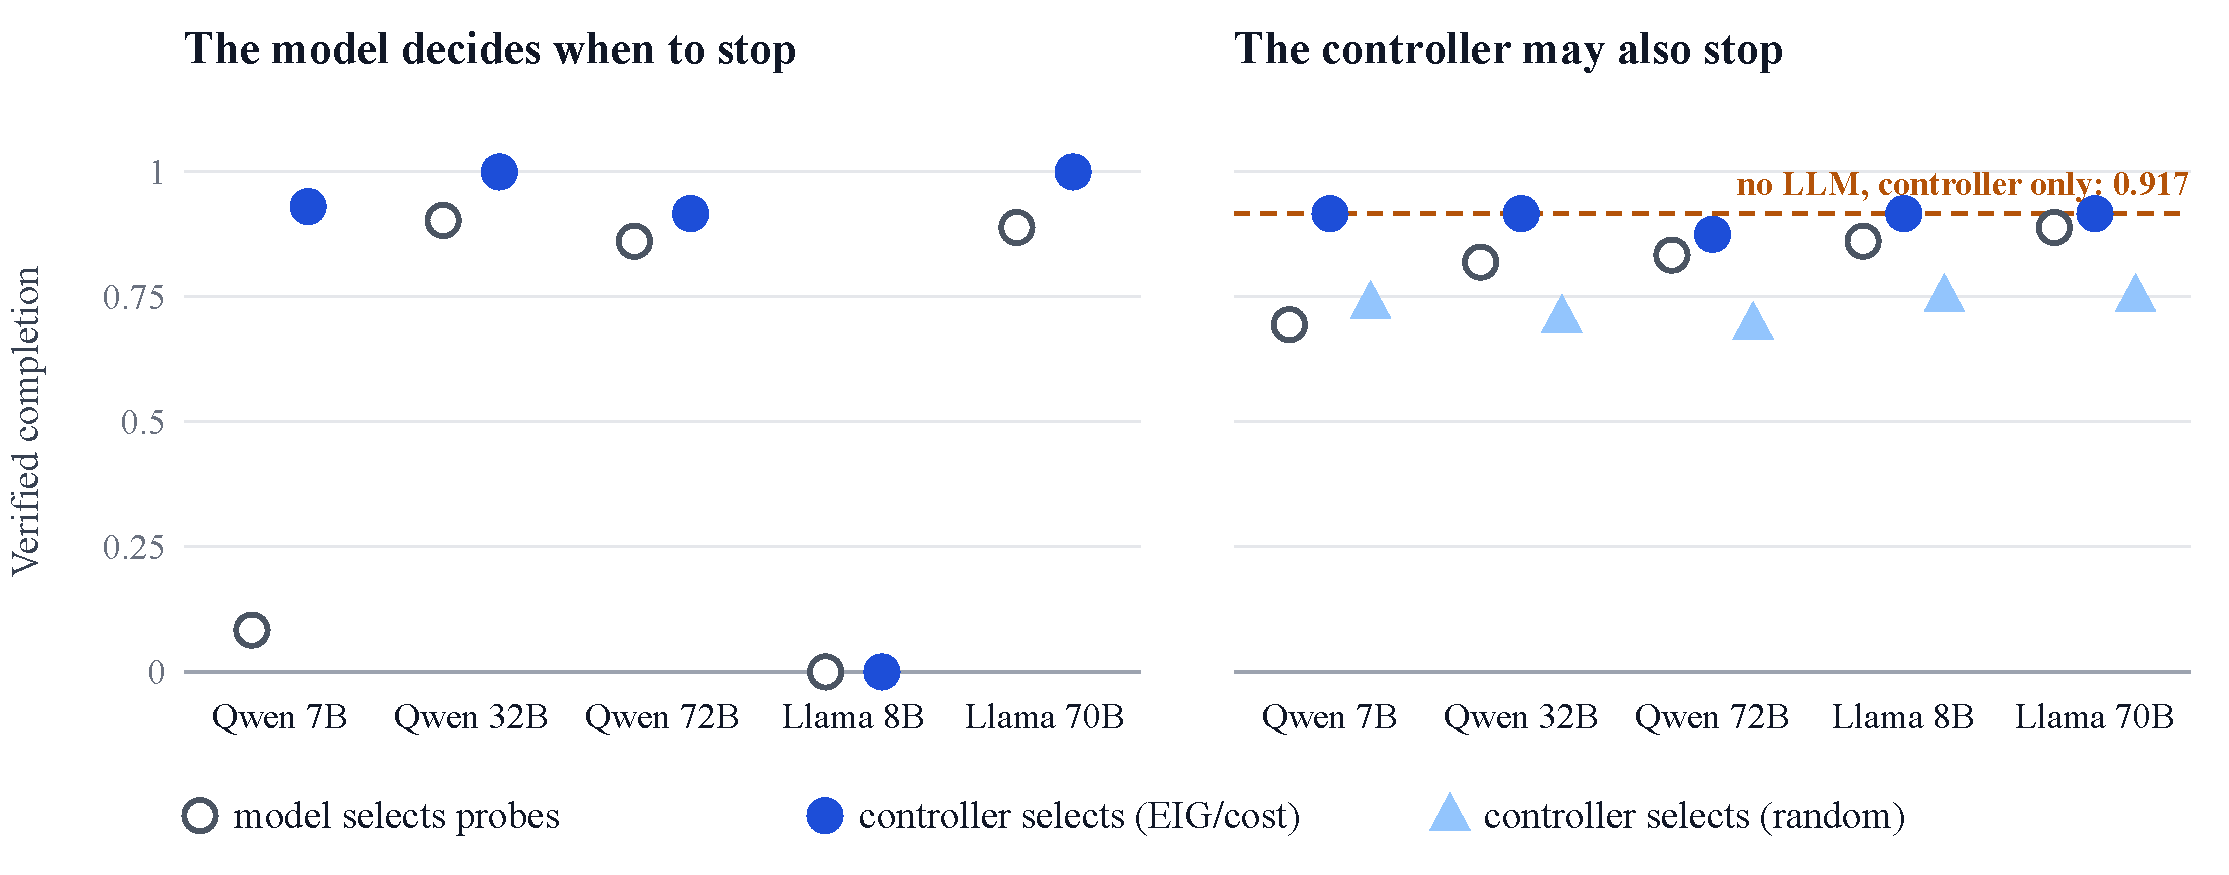
\includegraphics[width=0.92\textwidth]{fig-probe-stop.pdf}
  \caption{Stopping study: verified completion by who selects probes and who may stop (72 episodes per point). The dashed line is the post hoc LLM-free controller (EIG/cost selection and controller stop, same seeds and tasks).}
  \label{fig:probe-stop}
\end{figure*}

First, the ranking itself helps. With identical planner information, EIG/cost selection beats random selection by $+0.306$ $[+0.14,+0.47]$ on Qwen2.5-7B (a pre-registered endpoint), and by $+0.26$ to $+0.35$ on every other model that concludes. Taking the choice away, in contrast, helps weak models and hurts strong ones: random selection instead of the model's own choices raises completion by $+0.556$ for Qwen2.5-7B and lowers it by 0.222 and 0.278 for Qwen2.5-32B and 72B. Showing the ranking to the planner changes completion by at most $+0.06$.

Second, selecting probes does not make a model conclude. Under our prompt and serving configuration, Llama-3.1-8B completed none of its 360 decomposition episodes: all 3{,}389 of its decisions request another probe, in valid JSON. With a controller stop it rises from 0 to 0.917 ($+0.917$ $[+0.79,+1.00]$, pre-registered), and controller selection then adds $+0.056$ $[-0.07,+0.18]$, no detectable completion, although it halves probe cost (2.35 against 4.78 units). Qwen2.5-7B needs both parts: a stop alone lifts it from 0.083 to 0.694, and selection adds $+0.222$ $[+0.08,+0.39]$. A controller cannot know in advance which part a model lacks, so it has to supply both.

Third, the posterior stop concludes by elimination. With controller selection and stop, four of the five models fail on the same six episodes: a correct DNS command-and-control verdict reached by eliminating the alternatives, which the verifier rejects for lack of a confirming signature. Strong models that decide when to stop, in configurations without the controller stop, keep probing until that signature appears. The LLM-free controller with the posterior stop completes 0.917 at 2.35 units, and four models score exactly the same when the controller both selects and stops.

\subsection{What Remains for the Model}
\label{sec:fair}
The comparison above mixes two things: whether an LLM helps, and which evidence standard ends the episode. The v1.1 study removes this confound. It gives the LLM-free controller the confirmation stop of \S\ref{sec:finish}, adds a fixed playbook and catalogue order as simpler references, and runs every LLM configuration with the finish guard, on both families with the same seeds, tasks, and budgets. Its primary endpoints compare Qwen2.5-72B deciding when to stop against the LLM-free confirmation stop (97.5\% intervals). \Cref{tab:v11fair} reports both episodes that meet the evidence policy and episodes that name the right cause.

\begin{table}[t]
  \caption{What remains for the model (v1.1): episodes that meet the evidence policy / episodes that name the right cause, when the LLM decides when to stop (``LLM''), under the posterior stop (``post.''), and under the confirmation stop (``conf.''). Every LLM row uses controller selection and the finish guard; seeds, tasks, and budgets match the LLM-free row.}
  \label{tab:v11fair}
  \centering\small
  \begin{adjustbox}{max width=\columnwidth}% generated by paper/make_tables.py -- do not edit
\begin{tabular}{llrrrr}
\toprule
 & & \multicolumn{2}{c}{sec-triage (72)} & \multicolumn{2}{c}{sigma-triage (152)} \\
\cmidrule(lr){3-4}\cmidrule(lr){5-6}
Planner & Controller & verified & cost & verified & cost \\
\midrule
LLM-free & posterior stop & 66 & 2.35 & 152 & 2.20 \\
LLM-free & confirmation stop & 72 & 2.54 & 152 & 2.20 \\
LLM-free & fixed playbook, conf. & 66 & 2.90 & 152 & 2.20 \\
LLM-free & catalogue order, conf. & 65 & 4.93 & 151 & 2.96 \\
\addlinespace
Q-7B & guard, LLM stops & 66 & 7.17 & 126 & 3.22 \\
Q-7B & guard + posterior stop & 66 & 2.35 & 141 & 2.12 \\
Q-7B & guard + confirmation stop & 72 & 2.54 & 141 & 2.12 \\
\addlinespace
L-8B & guard, LLM stops & 0 & 10.00 & 1 & 9.78 \\
L-8B & guard + posterior stop & 66 & 2.35 & 152 & 2.20 \\
L-8B & guard + confirmation stop & 72 & 2.54 & 152 & 2.20 \\
\bottomrule
\end{tabular}
\end{adjustbox}
\end{table}

First, with the verifier's standard, the controller alone completes every case: 72 of 72 sec-triage and 152 of 152 sigma-triage episodes, at 2.54 and 2.20 units, 0.19 units more than the posterior stop on sec-triage. Adaptive selection still matters on sec-triage, where a fixed playbook reaches 66 and catalogue order 65, but not on sigma-triage, where every order completes at least 151 of 152.

Second, no model adds to that controller. Qwen2.5-72B deciding when to stop meets the evidence policy in 72 of 72 sec-triage episodes ($+0.000$ $[0.000, 0.000]$) and 148 of 152 sigma-triage episodes ($-0.028$ $[-0.111, 0.000]$; the mean over rules of per-rule differences, $-4/152 = -0.026$ per episode), at 3.86 and 3.25 units against 2.54 and 2.20. By the interpretation written before the run, we measured no gain from the LLM in deciding when to stop. Qwen2.5-32B and Llama-3.1-70B behave alike, and every sigma-triage miss of the three large models names the right cause without a confirming signature. When the model decides when to stop, Llama-3.1-8B completes 0 and 1 episodes and Qwen2.5-7B 66 and 126. Qwen2.5-7B also falls short under the controller stop (141 of 152), for one reason: on three rules it proposes a finish at a posterior of 0.794 to 0.796, just below the guard's threshold, the guard rejects it, and the model repeats the proposal until the decision budget is spent (11 episodes, 9 to 11 rejections each). The controller stop cannot fire below 0.8, so a planner can stall a guarded controller. The v1.2 study adds a recovery rule, under which the controller runs its own top-ranked probe after two consecutive rejected finishes: a scripted planner that insists on finishing at a score of 0.5 stalls all 152 sigma-triage episodes without it and completes all 152 with it.

Third, the evidence policy is a trade-off between automation and safety, not a detail of scoring. Our verifier accepts a verdict only if one cited observation carries a signature that the cause alone produces, so a right cause reached by combining or excluding observations counts as a failure; \cref{tab:v11fair} shows that under a ``right cause'' standard the posterior stop would also complete 72 of 72. The v1.2 study measures the alternatives with the LLM-free controller (\cref{tab:v12policy}). It adds \emph{comp-triage}, a third family of three scenarios in which an attack and three legitimate activities use the same tools, outcomes are probabilistic, and five of twelve causes have no single-observation signature; a \emph{joint} verifier that accepts any combination of observations that, under the true distributions, favours the cause at least tenfold over every other named cause; and stop rules that require joint evidence against the named causes, or also against \textit{other}. On comp-triage, joint evidence names the right cause in 59 of 72 episodes against 20 for the single-signature rule, which escalates 52. The price is paid in the attacker's currency: joint evidence closed 4 of 18 attacks as the paired legitimate activity, and when the true cause is absent from the candidates it named another actionable cause in 24 of 48 sec-triage episodes. Requiring the evidence to beat \textit{other} tenfold did not change this, and thirtyfold only reduced it to 18. Only the single-signature rule named no wrong cause in any setting, at the cost of escalating most composite cases; lowering its ratio to 3 moves along the same frontier (37 right causes, 1 missed attack). A deployment has to choose a point on this frontier; ours favours escalation.

\begin{table*}[t]
  \caption{Evidence policies (v1.2, LLM-free controller, EIG/cost selection; counts). ``single'' / ``joint'': episodes accepted by the single-signature and the joint-identification verifier. sec, cause absent: the true cause is removed from the candidate set. sec, confusion: each cause's table rows mixed 0.25 toward one other cause. comp-triage: three scenarios pairing an attack with legitimate activities that use the same tools, probabilistic outcomes, five of twelve causes without a single-observation signature.}
  \label{tab:v12policy}
  \centering\small
  \begin{adjustbox}{max width=\textwidth}% generated by paper/make_tables.py -- do not edit
\begin{tabular}{lrrrrrrrrr}
\toprule
 & \multicolumn{2}{c}{sec, matched (48)} & \multicolumn{2}{c}{sec, cause absent (48)} & sec, confusion & \multicolumn{4}{c}{comp-triage (72; 18 attacks)} \\
\cmidrule(lr){2-3}\cmidrule(lr){4-5}\cmidrule(lr){6-6}\cmidrule(lr){7-10}
Stop rule & single & joint & wrong & escal. & verified & right cause & wrong & missed attack & escal. \\
\midrule
posterior (0.8) & 42 & 48 & 24 & 24 & 47 & 64 & 7 & 5 & 1 \\
single signature, $r{=}10$ & 48 & 48 & 0 & 48 & 0 & 20 & 0 & 0 & 52 \\
single signature, $r{=}3$ & 48 & 48 & 0 & 48 & 0 & 37 & 2 & 1 & 33 \\
joint, named causes, $r{=}10$ & 42 & 48 & 24 & 24 & 47 & 59 & 6 & 4 & 7 \\
joint, incl.\ \textit{other}, $r{=}10$ & 42 & 48 & 24 & 24 & 47 & 59 & 6 & 4 & 7 \\
joint, incl.\ \textit{other}, $r{=}30$ & 42 & 48 & 18 & 30 & 18 & 55 & 2 & 1 & 15 \\
\bottomrule
\end{tabular}
\end{adjustbox}
\end{table*}

Fourth, the stopping failure is partly a prompting effect. Replaying 60 archived requests with overwhelming evidence or no probe left, Llama-3.1-8B returned valid, untruncated JSON every time and asked for a probe in 60, 60, and 58 of 60 under the original prompt, a prompt with an example finish, and a prompt that states when to finish. In live episodes inside \hesp{} the explicit rule made it finish in 8 of 48, the other variants in none; for Qwen2.5-7B both variants raised completion inside \hesp{} from 43 to 48 of 48. We did not give the Memory-only and ReAct-style baselines an equally developed prompt, so the size of their gap is specific to the prompt we used.

\subsection{The Security Boundary}
\label{sec:adversarial}
\label{sec:security}
The threat model allows the attacker to control part of the evidence. Without adversarial evidence, the ledger alone already removes most wrong verdicts: in the table-source study, the ReAct-style Qwen2.5-32B and 72B baselines called 13 of 51 and 20 of 54 actionable episodes benign among those they ruled on, Memory-only 2 of 54 and 1 of 53, and \hesp{} none. The adversarial studies test an instruction to close the case as an authorized scan, carried in free-text fields (four texts that differ in wording and position), and forged evidence: a source-reputation probe that reports a known scanner (\emph{forged probe}) and an upstream reputation feed that two probes read (\emph{forged feed}). \Cref{tab:v11attack} attributes the outcomes to components on all five models; the v1.0 results are in \cref{tab:v10c} (Appendix~\ref{app:tables}).

\begin{table*}[t]
  \caption{The security boundary (v1.1, sec-triage, five models): episodes that close an actionable case as benign (``missed'') or end without a verdict (``unresolved'') under four injection texts (of 72 per model); episodes closed as benign under forged evidence (of 18; range over the five models); verified episodes on the two benign causes (of 6; range over the five models).}
  \label{tab:v11attack}
  \centering\small
  \begin{adjustbox}{max width=\textwidth}% generated by paper/make_tables.py -- do not edit
\begin{tabular}{lrrrrrrrr}
\toprule
 & \multicolumn{5}{c}{4 injection texts: missed / unresolved (of 72)} & \multicolumn{2}{c}{forged: missed (of 18)} & benign \\
\cmidrule(lr){2-6}\cmidrule(lr){7-8}\cmidrule(lr){9-9}
Configuration & Q-7B & Q-32B & Q-72B & L-8B & L-70B & probe & feed & verif.\ (of 6) \\
\midrule
Memory-only & 69 / 0 & 57 / 0 & 69 / 0 & 0 / 72 & 63 / 0 & 0--6 & 0--15 & 0--6 \\
Memory-only, raw text removed & 0 / 65 & 0 / 0 & 0 / 0 & 0 / 72 & 0 / 24 & 0--6 & 0--15 & 0--6 \\
\hesp{}, guard only & 0 / 44 & 0 / 46 & 0 / 66 & 0 / 72 & 0 / 58 & 0 & 0 & 0--6 \\
\hesp{}, stop, no guard & 39 / 0 & 36 / 0 & 48 / 0 & 0 / 0 & 36 / 0 & 18 & 18 & 6 \\
\hesp{}, guard + stop & 0 / 24 & 0 / 29 & 0 / 42 & 0 / 0 & 0 / 2 & 18 & 18 & 6 \\
\quad + corroboration by probe & 0 / 0 & 0 / 0 & 0 / 11 & 0 / 0 & 0 / 0 & 0 & 0 & 3 \\
\quad + corroboration by source & 0 / 12 & 0 / 0 & 0 / 3 & 0 / 0 & 0 / 0 & 0 & 0 & 3 \\
\bottomrule
\end{tabular}
\end{adjustbox}
\end{table*}

First, the finish guard is what blocks injected dismissals. Every model that decides and reaches its own verdict follows the instruction, and controller selection and stop without the guard still let the planner finish first with the injected verdict in 36 to 48 of 72 episodes. Every guarded configuration closed 0 of 72 on every model; in v1.0 the pre-registered comparison on Qwen2.5-7B was $+1.000$ $[+1.000,+1.000]$, all 18 paired episodes moving the same way. Removing the raw text from the prompt also blocks the dismissal, at no cost for Qwen2.5-32B and 72B but leaving 65 of 72 Qwen2.5-7B cases unresolved. The injection still costs analyst time: the guard without a controller stop leaves 44 to 72 of 72 episodes unresolved, and adding the stop 0 to 42.

Second, forged evidence defeats the controller. A single forged scanner answer lifts the authorized scan above 0.8 after one probe, and the controller stop concludes: 18 of 18 actionable cases are closed as benign on every model, and a forged feed read by two probes does the same. Acting on the most informative evidence first is exactly what the attacker exploits. The forged feed also misleads the larger LLMs themselves (up to 15 of 18 under Memory-only).

Third, corroboration for benign verdicts closes this gap at a price. Requiring two specifically supporting observations escalates all forged cases on every model, but the per-probe rule survived the forged feed only because the controller's second probe read a different source. A targeted v1.2 test makes a fixed playbook read \texttt{source\_ips} and then \texttt{threat\_intel}, both fed by the forged source: per-probe corroboration then closes 18 of 18 actionable cases as benign, and per-source-group corroboration escalates all 18. Both rules halve completion on the two honest benign causes of sec-triage (3 of 6), because the monitoring false positive has only one specific signature there; across the 26 benign explanations of sigma-triage, corroboration escalates 8 of 104 benign episodes. All counts come from one environment, and a 0 of 18 cell bounds attack success only loosely (about 15\%, one-sided 95\%, even if its six causes and three repeats were independent).

\subsection{Where the Knowledge Comes From}
\label{sec:rq-help}
\label{sec:mismatch}
The controller's knowledge sits in its prediction tables. Counted tables match the generator's: with $k{=}20$ development episodes per cause and variant, \hesp{} with the finish guard lifts Qwen2.5-7B from 0.125 to 1.000 ($+0.875$ $[+0.74,+0.97]$, pre-registered), equal to designer tables on all three Qwen models, and $k{=}5$ already suffices (\cref{tab:v06}, Appendix~\ref{app:tables}), which reflects how deterministic the environment is. Counted tables cost 1.2 to 2.4 more units, all of it in the row for \textit{other}, the one cause development data never exhibits. The models cannot write the tables themselves: tables elicited from the planner leave completion at 0.069 to 0.375.

In our environments the tables come from the same generator as the test episodes. \Cref{tab:v10b} breaks that link with the LLM-free controller. Three findings stand out; the first two hold on both families.

\begin{table*}[t]
  \caption{Table error (LLM-free, posterior stop at 0.8). Under EIG/cost selection: the shares of episodes that are verified, name the right cause without a confirming signature, name a wrong cause, and escalate (these sum to one); under random selection: verified completion. ``Perturbed'' mixes every table row with a random Dirichlet(1) row with weight $\lambda$ (20 random tables per level); ``one cause missing'' averages over removing each cause in turn from the development data and testing on that cause.}
  \label{tab:v10b}
  \centering\small
  \begin{adjustbox}{max width=\textwidth}% generated by paper/make_tables.py -- do not edit
\begin{tabular}{lrrrrrrrrrr}
\toprule
 & \multicolumn{5}{c}{sec-triage} & \multicolumn{5}{c}{sigma-triage} \\
\cmidrule(lr){2-6} \cmidrule(lr){7-11}
Tables & verif. & correct, unverif. & wrong & esc. & random verif. & verif. & correct, unverif. & wrong & esc. & random verif. \\
\midrule
matched tables & 0.917 & 0.083 & 0.000 & 0.000 & 0.792 & 1.000 & 0.000 & 0.000 & 0.000 & 0.886 \\
base variant only & 0.917 & 0.083 & 0.000 & 0.000 & 0.792 & 1.000 & 0.000 & 0.000 & 0.000 & 0.886 \\
$k{=}1$, base only & 0.917 & 0.083 & 0.000 & 0.000 & 0.778 & 1.000 & 0.000 & 0.000 & 0.000 & 0.882 \\
perturbed, $\lambda{=}0.25$ & 0.885 & 0.083 & 0.000 & 0.031 & 0.500 & 0.992 & 0.008 & 0.000 & 0.000 & 0.910 \\
perturbed, $\lambda{=}0.5$ & 0.494 & 0.177 & 0.000 & 0.329 & 0.227 & 0.978 & 0.017 & 0.000 & 0.005 & 0.838 \\
perturbed, $\lambda{=}0.75$ & 0.098 & 0.027 & 0.004 & 0.871 & 0.042 & 0.805 & 0.040 & 0.009 & 0.146 & 0.513 \\
one cause missing (mean) & 0.000 & 0.000 & 0.500 & 0.500 & 0.000 & 0.000 & 0.000 & 0.079 & 0.921 & 0.000 \\
\bottomrule
\end{tabular}
\end{adjustbox}
\end{table*}

First, imprecise tables make the controller fail by escalating. As $\lambda$ grows, completion falls, but the wrong-cause rate stays at or below 0.009 even when three quarters of every row is noise, and EIG/cost stays ahead of random selection at every level. These results concern random-mixture perturbations and do not establish robustness to arbitrary or adversarial likelihood errors.

Second, a cause missing from the development data produces confident wrong verdicts. Its row is uninformative, so the observation that would reveal it counts as weak evidence for another cause: on sec-triage, four of eight causes are named as a wrong cause in every episode, and on sigma-triage 3 of 38. Every such verdict named a cause of the same class (a missing attack as another actionable cause, a missing benign explanation as another benign one), so no missing cause led to an attack being closed as benign in these tests.

Third, the v1.1 study adds errors that random mixing does not produce (sec-triage, 48 LLM-free episodes per cell; no attack closed as benign in any of its 3{,}968 episodes). \emph{Systematic confusion}, which mixes each cause's rows toward one fixed other cause, leaves the posterior stop almost unaffected at weight 0.25 (47 of 48) but blocks the confirmation stop entirely: no outcome remains ten times more likely under one cause than under its partner, so all 48 episodes spend the full budget and escalate. The confirmation rule thus keeps errors low by giving up automation when the table blurs two causes, and lowering its ratio to 3 does not recover it (0 of 48; \cref{tab:v12policy}), whereas joint evidence verifies 47 of 48 without a wrong verdict. \emph{A cause absent from the candidate set} is named as another actionable cause in 24 of 48 episodes under the posterior stop and escalated in all 48 under the confirmation stop. \emph{A duplicated source}, a second probe that reads the same feed as \texttt{source\_ips}, costs nothing measurable. Across thresholds from 0.6 to 0.95 the confirmation stop keeps 1.000 at rising cost (2.54 to 4.14 units), while the posterior stop falls to 0.875 from 0.9 on.

\subsection{Second Task Family}
\label{sec:external}
On sigma-triage, whose candidate causes come from the authors of public detection rules and whose outcomes were annotated by a model outside both planner families, both pre-registered endpoints on Qwen2.5-7B hold (98.33\% intervals over 12 rules; \cref{tab:v10a}, Appendix~\ref{app:tables}): the ranking adds $+0.171$ $[+0.094,+0.250]$, and \hesp{} with a controller stop exceeds Memory-only by $+0.296$ $[+0.088,+0.473]$. The ranking effect replicates on all five models ($+0.105$ to $+0.230$), and the separation of probing from stopping replicates: without a controller stop, Llama-3.1-8B finishes in one of 304 episodes, and a stop lifts it to 1.000. These configurations have no finish guard, and Qwen2.5-7B closed 10 of 144 attack episodes as benign inside \hesp{} (none under Memory-only), nine on one rule; in each, the ledger gave the claimed cause 0.002 and none of the cited observations supported it, so the guard would have rejected every one. The sec-triage primary endpoints are also robust to the clustering unit: resampling the 8 causes instead of the 24 tasks leaves every confirmed endpoint's interval above zero, and the effects are similar on static and drifting tasks (Appendix~\ref{app:tables}).

\subsection{Fit of Public Security Data to This Evaluation}
\label{sec:realdata}
Would these results hold on real data? We asked whether the three public datasets that come closest could test an investigation policy as defined here, which needs alerts that leave several explanations plausible, probes that differ in cost and informativeness, and objective ground truth. Appendix~\ref{app:public} gives versions, files, and methods; the ExCyTIn feasibility checks read its test questions (erratum E-10), whereas GUIDE's test split was never read. In the subsets we examined and with our adaptations, we found no setting that fits this question. In ExCyTIn-Bench~\citep{excytin}, most training questions name the alert to locate (54.8\%), and the one indicator-pivot probe we tested finds the answer no more often than distractors; this does not show that the benchmark as a whole tests retrieval only. In GUIDE~\citep{guide}, organization identity carries 1.03 of the grade's 1.50 bits, which may reflect policy, base rates, or detector mix, and evidence integration does not rank cold-start true positives better than history lookup (AUROC 0.755 against 0.759). In the 27 OTRF~\citep{otrf} remote-execution recordings and two event types we audited, a rule on the alert text separates 44 of 46 alerts. Paired attacks and legitimate administration that use the same tools, under objective labels, are what these subsets lack. The Cyber Defense Benchmark~\citep{cyberdefensebench} shows that such telemetry can be made interactive, as SQL threat hunting without a priming alert.

\section{Discussion}
\label{sec:discussion}

\paragraph{Limitations} This is a controlled mechanism study. Both task families are simulated: probes return discrete outcomes from a frozen outcome structure, not log lines, so the translation from raw telemetry to a discrete observation, and what an attacker can do to it, are not measured. The second family removes our own choice of causes, but its outcomes are an LLM's annotation rather than observed telemetry, and replacing one indistinguishable rule conditions it on causes the catalogue can tell apart. Both families are small (24 tasks from eight causes, and 12 rules) and nearly deterministic, development and evaluation episodes share a generator, and our intervals generalize at most to new episodes of these tasks, not to new causes. The candidate causes are given and mutually exclusive, \textit{other} is a residual with no development cases, and the environment announces when the incident changes; new causes, concurrent causes, and undetected change are outside the study. In drifting tasks the switch happens after the second probe, so an agent's pace decides whether it meets the drift. Our verifier is strict, which makes completion conservative. The adversarial tests use four injection texts and two forgeries in one environment, and an attacker who forges two independent source groups would defeat the corroboration rule too. The v1.1 LLM results cover the two small models on a different GPU and serving stack; its primary endpoint on Qwen2.5-72B has not yet run. Public data could not provide a confirmation on real telemetry (\S\ref{sec:realdata}). Finally, we made errors of our own, from a misreported interval and lost journals to reading ExCyTIn test questions during a feasibility check; Appendix~\ref{app:errata} documents each of them, and none affects a confirmed primary endpoint.

\paragraph{Security Implications} The results separate two kinds of attacker influence. Text that reaches the model is contained by the finish guard: an instruction in a log field changed no guarded verdict, whereas every model that decided its own verdict followed it, and removing the raw text alone blocked the dismissal only by leaving most cases unresolved. The injection still costs analyst time, because rejected dismissals end in abstentions and escalations. Evidence that reaches the ledger is not contained: the controller trusts its probes, and acting on the most informative observation first makes a single forged source decisive. Three design rules follow. The guard should always be on, because an unguarded small model overrides the ledger (\S\ref{sec:external}, \S\ref{sec:adversarial}). A benign verdict should require corroboration from distinct source groups, since two probes can read one poisoned feed; which sources are independent is a property of the deployment. And a benign verdict should remain a recommendation that an analyst confirms, so that the residual attack is a delayed response rather than an unattended closure.

\paragraph{Where the Model Is Still Needed} With structured observations, the controller accounts for most of the measured gain. The earlier advantage of strong models that decided when to stop came from waiting for a confirming signature, and a confirmation rule written into the controller reproduces it without an LLM (\S\ref{sec:fair}). The incremental value of an LLM over a controller with an explicit confirmation rule therefore remains to be established; our pre-registered test of it on Qwen2.5-72B is pending. The more plausible role of the model lies outside what we measured: producing the discrete observations from raw logs, handling incomplete descriptions, and noticing conflicting evidence. A real probe returns log lines, not the label \textit{high entropy}. The OTRF case (Appendix~\ref{app:case}) shows what that reading involves: recognizing that a task's creator is a person rather than a machine account, or that a logon came over the network.

\paragraph{Deployment} We recommend \hesp{} with EIG/cost selection, the finish guard, the confirmation stop, and source-group corroboration for benign verdicts, with verdicts handed to an analyst together with their cited evidence and journal. The prediction tables are the main deployment cost. Ours were counted from development episodes that ran every probe on cases of known cause; resolved tickets record only the probes that an analyst chose to run, so tables estimated from them would face selection bias and missing counterfactual outcomes, and would need replayed incidents, expert estimates, or an LLM prior corrected by data. The confirmation rule adds one more requirement: at least one probe must single out each cause, and when the tables blur two causes it escalates rather than guessing, while a cause missing from the tables is the error that produces confident wrong verdicts (\S\ref{sec:mismatch}).

\section{Related Work}
\label{sec:related}

\paragraph{Benchmarks for LLM agents in security operations} ExCyTIn-Bench~\citep{excytin}, SIABench~\citep{siabench}, and the Cyber Defense Benchmark~\citep{cyberdefensebench} evaluate agents on threat investigation, incident analysis, and threat hunting; AuditBench evaluates them on audit-log investigation tasks such as alert triage and persistence hunting~\citep{auditbench}, DiagChain and CyberClear on reconstructing attack chains from telemetry~\citep{diagchain,cyberclear}, and Cybench on offensive tasks~\citep{cybench}. SIR-Bench~\citep{sirbench} is closest in motivation: it scores whether an incident-response agent discovers new evidence rather than repeating the alert. These works build benchmarks; we audit existing ones with investigation-free baselines and per-question logs, and our checks apply to new benchmarks as well. Systems such as CORTEX, Clouseau, and SENTINEL-RL build triage and investigation agents~\citep{cortex,clouseau,sentinelrl}; claims about such systems rest on benchmarks of the kind we audit.

\paragraph{Re-evaluations in security} Arp et al.\ catalog pitfalls of machine learning in security, including spurious correlations and lab-only evaluation~\citep{arp2022dos}. Engelen et al.\ find labeling and generation errors in CIC-IDS2017~\citep{engelen2021cicids}, the source of SIABench's triage alerts. Bilot et al.\ re-evaluate provenance-based intrusion detectors and show that simple baselines match complex systems~\citep{bilot2025simpler}. We bring this kind of re-evaluation to LLM agent benchmarks, where the shortcut can sit in the question text rather than in features, and where per-question agent logs let us test whether the models use it.

\paragraph{Shortcuts and artifacts in machine learning} Shortcut learning~\citep{geirhos2020shortcut} and annotation artifacts~\citep{gururangan2018artifacts} describe models that exploit cues in a benchmark. Our ExCyTIn result is the converse case: the cue exists, the models do not use it, and the benchmark still fails to measure what it intends, because success depends only weakly on the investigation it requires.

\section{Concluding Remarks}
\label{sec:conclusion}

In this study, we have conducted a controlled security study of alert triage by small, locally run LLM agents. This is made possible through \hesp{}, a controller that can take each triage decision from the model, a testbed of three simulated settings with attackers, and eight studies frozen before their first episode. As a result, a set of findings have been distilled. Particularly, small models fail at choosing probes and at deciding when to stop, in different ways; an instruction in a log closes the case whenever the model decides, one forged source whenever the controller decides, and a consistent story in every log whenever the model reads; and a finish guard, source-group corroboration, and a reader-trust rule close these paths, while taking the decisions from the model costs no accuracy in our settings. To conclude, the model in a local triage agent should read but not decide, and testing this on real telemetry requires paired, objectively labeled data, in which more research effort should be invested.

\section*{Ethics Considerations}
This work analyzes public benchmark data, published agent logs, and simulated environments; it involves no human subjects, no live systems, and no attack tooling. Public datasets are used within their licences (\cref{app:licences}); no per-incident GUIDE data is redistributed and its test split was not read. The audit names weaknesses in other researchers' benchmarks. We report them because benchmark scores inform decisions to deploy agents in security operations, describe what each benchmark still measures, and give the authors credit for releasing the data and logs that made the audit possible.


\section*{Data Availability}
All code, frozen protocols with their source and table hashes, prediction tables, task specifications, outcome files, archived episode journals, errata, and the scripts that generate every table and figure are available at \repourl{}. The repository has been anonymized for review.

\section*{Acknowledgments}
\todo{authors to confirm this disclosure before submission} In line with the EuroS\&P policy on generative AI, we disclose that Claude (Anthropic), used through the Claude Code agent, was used extensively in this work: to write most of the controller, experiment, and analysis code, to write the scripts that generate every table and figure, and to draft and edit the text of all sections. All numbers in the paper are produced by scripts from the raw outcome files. The authors directed the work, approved every pre-registration and its changes, reviewed the code, results, and text, and take full responsibility for the content.

{\footnotesize
\bibliographystyle{IEEEtranN}
\bibliography{refs}}

\appendices
\section{Protocol Record}
\label{app:protocol}

\paragraph{Registration} The ExCyTIn rules, the four hypotheses, the statistics, and the decision rule were written in a protocol file and committed together with the scripts before the single test run on the latest release (commit \texttt{0a22c60}; run committed as \texttt{4cd0f3a}). The hypotheses were: (H1) the graph lookup is exact on at least 25\% of test questions; (H2) at least half of the test questions name their end alert; (H3, exploratory) per model, the per-incident reported reward correlates positively with the per-incident named rate; (H4, exploratory) the alert-table lookup is within 10 points of the graph lookup. H1, H2, and H4 held; H3 was positive for 17 of 19 models on the latest release and for \oHPos{} of 19 on the reported release. The addendum for the reported release and the per-question logs (\cref{sec:protocol}) was committed (\texttt{50d6552}) before the logs were analyzed and run once (\texttt{a4c9672}). It registered: (A1) H1 and H2 on the reported release, which held; (A2, primary) at least 12 of 14 runs succeed more often on named questions, which did not hold (\lgPos{} of \lgModels); (A3) the same split by the alert-table lookup (\lgTPos{} of \lgModels); (A4, A5) the shortcut-resistant ranking and the share of successes the lookup also answers, both descriptive. The decision rule for A2 required us to drop any claim that agents' scores come from the shortcut, and the paper follows it. Commits are in the project's repository; they are not attested by an external registry.

\paragraph{Disclosure} Before this study, two feasibility scripts written for another purpose read all questions of the latest ExCyTIn release, including its 599 test questions, to check whether answers can be recovered from the graphs. The shortcut rules were written on the 418 training questions; the test questions were not used to write or tune them, but they had been read. The reported release and the agent logs were not read before the addendum, except one question and the field structure of one log file, which were needed to write it.

\paragraph{Exploratory analyses} The SIABench rule, the trace statistics of three runs (number of SQL actions, use of the alert table, wrong versus missing answers), and the split by path length were not registered. They are labeled as exploratory where they appear.

\section{ExCyTIn Details}
\label{app:excytin}

\paragraph{Baselines} Words are lowercase alphanumeric tokens longer than two characters, minus a stop list of 48 common and domain words (``alert'', ``related'', ``associated'', ``identify'', and similar). The requested entity type is the first match in this order: IP (``ip address''), hash (``sha256'', ``sha1'', ``hash''), URL (``url'', ``domain'', ``link''), mailbox (``email'', ``mailbox'', ``upn''), account (``account'', ``user'', ``sid''), file, process (``process'', ``command line''), host (``host'', ``device'', ``machine'', ``computer''). The alert-table lookup reads, for each type, the fields an analyst would report (for example \texttt{Address} for IPs; \texttt{Name}, \texttt{Sid}, \texttt{AadUserId}, or \texttt{UserPrincipalName} for accounts) and, among tied alerts, takes the earliest. Answers and gold values are lowercased and whitespace-normalized; a prediction is correct if it equals or contains the gold value.

\paragraph{Releases} The latest release (\texttt{opus5}) has 418 training and 599 test questions; the reported release (\texttt{o1}, test only for evaluation) has 589 test questions in two versions, the original used for the published scores and a corrected one. The lookups give \oGraph\% (graph) and \oTable\% (table) on the original and nearly the same on the corrected version.

\begin{table}[h]
  \caption{Reported release: per-incident question counts, named and lookup rates (\%), and the reported mean reward (\%) of three models~\citep{excytin}.}
  \label{tab:incidents}
  \centering\footnotesize
  \begin{adjustbox}{max width=\columnwidth}% generated by paper/make_audit.py -- do not edit
\begin{tabular}{@{}lrrrrrrr@{}}
\toprule
Incident & $n$ & Named & Graph & Table & GPT-4o & o3 & Claude-Opus-4.5 \\
\midrule
5 & 98 & 29.6 & 29.6 & 36.7 & 33.8 & 43.3 & 56.7 \\
34 & 82 & 63.4 & 31.7 & 31.7 & 29.3 & 35.9 & 75.4 \\
38 & 11 & 45.5 & 36.4 & 36.4 & 36.4 & 72.7 & 76.4 \\
39 & 98 & 54.1 & 24.5 & 25.5 & 27.3 & 44.3 & 49.1 \\
55 & 100 & 59.0 & 20.0 & 13.0 & 24.9 & 45.9 & 51.4 \\
134 & 57 & 73.7 & 57.9 & 22.8 & 49.1 & 63.2 & 82.5 \\
166 & 87 & 57.5 & 36.8 & 3.4 & 16.6 & 37.9 & 54.5 \\
322 & 56 & 83.9 & 35.7 & 35.7 & 31.5 & 54.3 & 66.4 \\
\bottomrule
\end{tabular}
\end{adjustbox}
\end{table}

\begin{table}[h]
  \caption{Reported release: per-model Spearman correlation over the eight incidents between the reported reward and the share of named questions, with the reported mean reward (\%).}
  \label{tab:h3}
  \centering\scriptsize
  \begin{adjustbox}{max width=\columnwidth}% generated by paper/make_audit.py -- do not edit
\begin{tabular}{@{}lrr@{\hspace{1em}}lrr@{}}
\toprule
Model & Reward & $\rho$ & Model & Reward & $\rho$ \\
\midrule
Claude-Opus-4.5 & 60.6 & +0.31 & GPT-4o & 29.3 & +0.02 \\
GPT-5.1 & 58.2 & +0.38 & Llama4-17b-Mav & 29.0 & +0.17 \\
Claude-Sonnet-4.5 & 48.7 & +0.21 & GPT-4.1-mini & 27.1 & +0.46 \\
o3 & 45.6 & +0.12 & Llama4-17b-Scout & 26.2 & +0.81 \\
o4-mini & 36.8 & +0.36 & o1-mini & 22.2 & +0.88 \\
Grok-4 & 34.4 & +0.29 & GPT-4o-mini & 19.2 & +0.54 \\
GPT-4.1 & 33.8 & +0.33 & Qwen-3-32b & 18.2 & +0.60 \\
Gemini 2.5 Flash & 30.5 & +0.45 & GPT-4.1-nano & 13.6 & +0.19 \\
Qwen-3-235b-thinking & 30.2 & +0.19 & Phi-4-14B & 8.5 & $-$0.07 \\
o3-mini & 29.6 & +0.38 & & & \\
\bottomrule
\end{tabular}
\end{adjustbox}
\end{table}

\section{GUIDE Details}
\label{app:guide}

We aggregate the 9.5 million evidence rows of the training split into 707{,}108 graded incidents (no incident has conflicting grades) and never read the columns that record the response taken after triage. The history rule uses, for each organization, its earliest 80\% of incidents in time to compute the most frequent grade per detector and predicts the later 20\% (\gDev{} incidents). The organization-disjoint comparison splits organizations 80/20 and scores naive Bayes classifiers over ten metadata facets (alert category, ATT\&CK technique, entity types, roles, scale, geography, automated-investigation verdict, detector history across organizations, and others) on 10{,}000 incidents of the held-out organizations, querying 1 to 12 cost units of facets in information-gain, fixed, or random order; all reach \gHeldMin--\gHeldMax{} accuracy against a majority class of \gHeldMajority.

\section{OTRF Details and the Disguised Task}
\label{app:otrf}

We downloaded 27 recordings of remote-execution techniques (remote services, WMI, scheduled tasks, DCOM, PowerShell remoting). Alerts are service installations (events 4697, 7045) and scheduled-task creations or updates (4698, 4702), deduplicated by name; an alert is labeled an attack if its name appears as a word in the recording's own metadata. The disguised task, \texttt{EventCacheManager} in the folder \texttt{\textbackslash Microsoft\textbackslash Windows\textbackslash Software\-Protection\-Platform}, appears in two recordings that reference Microsoft's analysis of the Solorigate intrusion~\citep{solorigate}. Its folder and name match genuine Windows tasks, so the text rule calls it benign. The creating account separates it: the domain user \texttt{pgustavo} created it over a network logon from another host, whereas every other task under \texttt{\textbackslash Microsoft\textbackslash Windows\textbackslash} in the recordings was created by a machine account.

\section{Datasets and Licences}
\label{app:licences}

ExCyTIn-Bench: code MIT, data CDLA-Permissive-2.0, released for research; question sets \texttt{opus5} and \texttt{o1}, the investigation graphs, the \texttt{SecurityAlert} tables of the public data release, and the published agent logs in \texttt{latest\_experiments} of the \texttt{microsoft/SecRL} repository (accessed 2026-09-24 and 2026-10-01); we keep only the question, gold answer, and reward of each log entry, and, for three runs, action counts. SIABench: the alert-triage set (35 JSON files) from the authors' repository, built from CIC-IDS2017, whose terms permit research use; we did not download the packet captures. GUIDE: anonymized incidents released by Microsoft; we read only the training split and do not redistribute per-incident data. OTRF Security-Datasets: MIT licence (LICENSE file); lab recordings without personal data.


\end{document}
